\hypertarget{network-address-translation-nat}{%
\chapter{Network Address Translation
(NAT)}\label{network-address-translation-nat}}

\begin{figure}
\centering
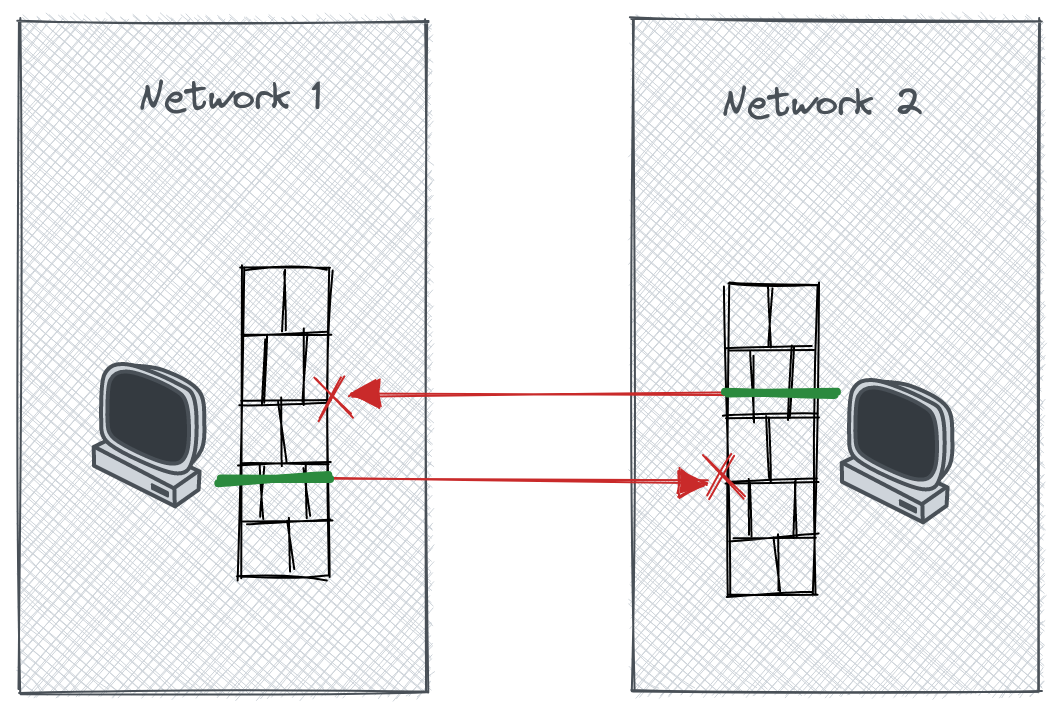
\includegraphics[width=\textwidth,height=0.66\textheight]{presentation/../figures/nat-intro.png}
\caption{``Two parties behind separate NATs''\label{nat-intro}}
\end{figure}

\begin{itemize}
\tightlist
\item
  Parties behind a NAT device (usually their router)

  \begin{itemize}
  \tightlist
  \item
    Can initiate a connection to a public endpoint
  \item
    Cannot be discovered from the outside
  \item
    Neither party can initiate the connection to the other
  \end{itemize}
\end{itemize}
